
\documentclass[a4paper,UKenglish,cleveref, autoref, thm-restate]{lipics-v2021}

\usepackage{amsmath,amssymb,amsthm}
\usepackage{stmaryrd}
\usepackage{proof}
\usepackage{tikz}
	\usetikzlibrary{calc}

\usepackage{FMC}


\bibliographystyle{plainurl}


% - - - - - - - - - - - - - - -


%\newcommand\looppicx[1]{
%\begin{tikzpicture}[thick,x=12pt,y=12pt,outer sep=0pt,inner sep=2pt]
%	\coordinate (m) at (0,0);
%	
%	\begin{scope}[->,>=stealth,anchor=north]
%		\ifx#11
%		\draw (m)--node[pos=0.6,anchor=east]{$\termcolor\scriptstyle{i\vphantom j\,}$} (-1,-2) node {$\vphantom:\typecolor\scriptstyle{p}$};
%		\draw (m)--node[pos=0.6,anchor=west]{\,$\termcolor\scriptstyle{j}$}            ( 1,-2) node {$\vphantom:\typecolor\scriptstyle{q}$};
%		\else
%		\draw (m)--node[pos=0.6,anchor=east]{$\termcolor\scriptstyle{i\vphantom j\,}$} (-1,-2) node {$\vphantom:\typecolor\scriptstyle{\frac p{1-q}}$};
%		\fi
%	\end{scope}
%	
%	\node (x) at (0,-3) {};
%	
%	\coordinate (a) at ( .85,-1.7);% \node[gray,circle,draw,inner sep=0pt,minimum size=2pt] at (a) {};
%	\coordinate (b) at (1.25,-1.6);% \node[gray,circle,draw,inner sep=0pt,minimum size=2pt] at (b) {};
%	
%    	\ifx#10
%		%\draw (m) [rounded corners=20pt] -- (1.25,-2.5) [rounded corners=5pt] -- (1.25,1.5) -- (0,1.5) -- (0,1);
%		\draw[rounded corners=5pt] (m) -- (.5,-1) .. controls (a) and (b) .. (1.25,-.75) -- (1.25,1.5) -- (0,1.5) -- (0,1);
%    	\fi	
%	
%	\node[draw=red,fill=red!10,rounded corners,minimum size=16pt] (M) at (m) {$\term M$};
%	\draw[->,>=stealth] (0,2)--(M);	
%\end{tikzpicture}
%}

\newcommand\looppic[1]{
\vcenter{\hbox{%
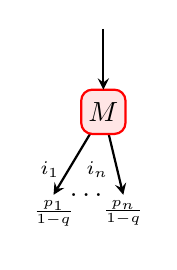
\begin{tikzpicture}[thick,x=18pt,y=15pt,outer sep=0pt,inner sep=2pt]
	\coordinate (m) at (0,0);
	
	\node at (-0.3,-2) {$\dots$};
	
	\begin{scope}[->,>=stealth,anchor=north]
		\draw (m)--node[pos=0.7,anchor=east]{$\termcolor\scriptstyle{i_1\,}$} (-1,-2) node {$\vphantom:\typecolor\scriptstyle{\ifx#11p_1\else\frac{p_1}{1-q}\fi}$};
		\draw (m)--node[pos=0.7,anchor=east]{$\termcolor\scriptstyle{i_n\,}$} (.4,-2) node {$\vphantom:\typecolor\scriptstyle{\ifx#11p_n\else\frac{p_n}{1-q}\fi}$};
	\ifx#11
		\draw (m)--node[pos=0.7,anchor=west]{\,$\termcolor\scriptstyle{j}$}   ( 1,-2) node {$\vphantom:\typecolor\scriptstyle{q}$};
	\fi
	\end{scope}
	
	\node (x) at (0,-3) {};
	
	\coordinate (a) at ( .85,-1.7);% \node[gray,circle,draw,inner sep=0pt,minimum size=2pt] at (a) {};
	\coordinate (b) at (1.25,-1.6);% \node[gray,circle,draw,inner sep=0pt,minimum size=2pt] at (b) {};
	
    	\ifx#10
		%\draw (m) [rounded corners=20pt] -- (1.25,-2.5) [rounded corners=5pt] -- (1.25,1.5) -- (0,1.5) -- (0,1);
		\draw[rounded corners=5pt] (m) -- (.5,-1) .. controls (a) and (b) .. (1.25,-.75) -- (1.25,1.5) -- (0,1.5) -- (0,1);
    	\fi	
	
	\node[draw=red,fill=red!10,rounded corners,minimum size=16pt] (M) at (m) {$\term M$};
	\draw[->,>=stealth] (0,2)--(M);	
\end{tikzpicture}}}
}

\newcommand\heads{\mathsf{h}}
\newcommand\tails{\mathsf{t}}
\newcommand\PFMC{FMC^\oplus}
\renewcommand\eval[5]{#1,#2,\term{#3}\,\evalarrow\,#4,\term{#5}}
\newcommand\Eval[3]{#1,\term{#2}\,\evalarrow\,#3}
\newcommand\pr[1]{\mathsf{pr}(#1)}
\newcommand\ret[2]{#1[#2]}

%==================================================================================================== FRONTMATTER

\title{Simple Types for Almost Sure Termination}

\author{Ugo {Dal Lago}}{University of Bologna, Italy \and INRIA Sophia Antipolis, France}{ugo.dallago@unibo.it}{https://orcid.org/0000-0001-9200-070X}{}

\author{Willem Heijltjes}{University of Bath, United Kingdom \and \url{http://willem.heijltj.es}}{w.b.heijltjes@bath.ac.uk}{https://orcid.org/0009-0001-8941-1150}{}

\authorrunning{U. Dal Lago and W. Heijltjes}

\Copyright{Ugo Dal Lago and Willem Heijltjes}

\ccsdesc[500]{Theory of computation~Lambda calculus}
\ccsdesc[300]{Theory of computation~Probabilistic computation}

\keywords{probabilistic lambda-calculus, type systems, almost sure termination}

%\relatedversion{}

%\acknowledgements{Georgina Majury?}

\nolinenumbers

\EventEditors{}
\EventNoEds{0}
\EventLongTitle{}
\EventShortTitle{}
\EventAcronym{}
\EventYear{}
\EventDate{}
\EventLocation{}
\EventLogo{}
\SeriesVolume{}
\ArticleNo{}

%==================================================================================================== DOCUMENT
\begin{document}

\maketitle

\begin{abstract}

\end{abstract}
   
%---------------------------------------------------------------------------------------------------- INTRODUCTION

\section{Introduction}

We are interested in applying the tools of the $\lambda$-calculus, in particular confluent reduction and type systems, to probabilistic computation. In~\cite{DalLago-Guerrieri-Heijltjes-2020} we restored confluence to a probabilistic $\lambda$-calculus, the probabilistic event $\lambda$-calculus (PEL), by decomposing probabilistic choice into a \emph{sampling} construct and a \emph{conditional}. Independently in~\cite{Antonelli-DalLago-Pistone-2022} and~\cite{Heijltjes-Majury-2025}, from different inspirations we converged on essentially the same probabilistic type system for the PEL to give lower bounds on the probability of termination. In this paper we further extend the calculus, and develop a type system for \emph{almost sure termination} (AST): termination with probability one.

We start from the following observation. \emph{Iteration}, generally represented by while-loops, repeats a given function $f$ until a condition is fulfilled. In the typed case, illustrated  below, the function $f$ is required to return a sum $B+A$ where the choice between returning a value $A$ or $B$ represents the condition. Then $\mathsf{iter}\,f$ first evaluates $f$, and exits on $B$ and repeats on $A$.
\[
\begin{array}{@{}r@{}l@{}}
	f &{}: A \to B+A
\\ \hline
	\mathsf{iter}\,f &{}: A\to B
\end{array}
	%\infer{\mathsf{iter}~f : A\to B} { f : A \to B+A } 
	% \qquad \mathsf{iter}~f~=~[\mathsf{id},\mathsf{iter}~f]\,\circ\,f
	%It is defined as the least solution to the equation below right, where $[-,-]$ is the co-diagonal of the coproduct.
\]
We observe that if we replace $B+A$ by a probabilistic sum $B \oplus_p A$ with a fixed probability $p\in (0,1]$, i.e.\ the probability of choosing $B$ is non-zero, then $\mathsf{iter}\,f$ is \emph{almost surely terminating} (provided of course that $f$ is itself terminating). This opens a way to approach almost sure termination via type systems.

These considerations illustrate how probabilistic choice is connected to other imperative features such as sequentiality and iteration. Derived from the PEL, the second author has developed new approach to unifying the $\lambda$-calculus with imperative computation and effects, the \emph{Functional Machine Calculus} (FMC)~\cite{Heijltjes-2023}. Its most recent iteration~\cite{Heijltjes-2025-MFPS} features branching sequential computation and iteration, providing an ideal vehicle for our present study.

In the FMC each branch of the computation is labelled with a \emph{choice} label $i,j,k,\dots$, which takes the role of a constant, an exception, a case label, or an exit status. For example, the boolean constants $\bot$ and $\top$ are choice labels. Iteration of a term $\term M$ is written $\term{M^i}$, which evaluates $\term M$ and repeats if $\term M$ chooses $i$, and terminates for any other choice. The calculus encodes a fair probabilistic choice, which we write as $\term{M+N}$.

\begin{example}
The term $\term{(\heads + (\tails + \,i))^i}$ chooses \emph{heads}, the choice label $\heads$, with probability $\frac12$, \emph{tails} $\tails$ with probability $\frac14$, and iterates with probability $\frac14$, to give an overall probability of $\frac 23$ for $\heads$ and $\frac 13$ for $\tails$. We illustrate it pictorially as follows.
\[
	\term{(\heads + (\tails + \,i))^i}
\quad=\quad
\vcenter{\hbox{%
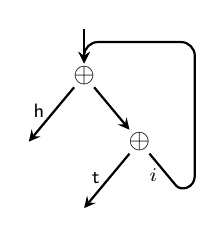
\begin{tikzpicture}[thick,x=20pt,y=24pt,outer sep=0pt,inner sep=1pt]
	\node (x) at (1,2) {$\termcolor\oplus$};
	\node (y) at (2,1) {$\termcolor\oplus$};

	\coordinate (a) at (2.75,0.25); %\node[gray,circle,draw,inner sep=0pt,minimum size=2pt] at (a) {};
	\coordinate (b) at (3   ,0.3);  %\node[gray,circle,draw,inner sep=0pt,minimum size=2pt] at (b) {};
	
	\begin{scope}[->,>=stealth,anchor=north]
	
	\draw (1,2.7)--(x);
	\draw (x)--(y);
	\draw (x) --node[pos=0.6,anchor=south east]{$\termcolor\scriptstyle{\heads}$} (0,1);
	\draw (y) --node[pos=0.6,anchor=south east]{$\termcolor\scriptstyle{\tails}$} (1,0);
	
	\draw[rounded corners=5pt] (y) -- node[pos=0.6,anchor=north east]{$\,\termcolor\scriptstyle{i}$}  
	  (2.5,0.5) .. controls (a) and (b) .. (3,0.7) -- (3,2.5) -- (1,2.5) -- (x);
	\end{scope}
\end{tikzpicture}}}
\]
\end{example}

The type system, simplified for this introduction to omit return values, records the probability of terminating with each given choice. A term $\term M$ is typed as follows, indicating that it may choose $i_k$ with probability $p_k$ from choices $i_1$ through $i_n$.
\[
	\term{M : \e ~=>~ p_1 i_1 + \cdots + p_n i_n }
\]
Here, the double arrow $\type{=>}$ is the function type and $\type\varepsilon$ represents the lack of an input value. The return type is a probability (sub-)distribution over the choices $\{i_1,\dots,i_n\}$, written as a formal sum. The probabilities $p_1$ through $p_n$ may sum to less than one, with the remainder representing a probability of divergence.

\begin{example}
The body of our example term, without the loop, has the following type.
\[
	\term{\heads + (\tails + \,i) : \e ~=>~ /12\heads + /14\tails + /14i}
\]
\end{example}

Iteration $\term{M^i}$ removes the choice $i$ from the possible return choices. In the probabilistic setting, the remaining probabilities must then be renormalized to form a distribution. That is, if $i$ has probability $q$, the remaining choices (including divergence) have a total probability of $1-q$, and must be multiplied by $\frac1{1-q}$ to return the total to one. Typing for iteration is then as follows.
\[
\begin{array}{@{}r@{}l@{}}
	\term{M}   &{}: \type{\e ~=>~ p_1i_1 + \dots + p_ni_n + qj}
\\ \hline \\[-10pt]
	\term{M^j} &{}: \type{\e ~=>~ /{p_1}{1-q}i_1 + \dots + /{p_n}{1-q}i_n}
\end{array}	
\qquad
\term{M}=\looppic1 \qquad \term{M^j}=\looppic0
\]

\begin{example}
The return type for our example term is given by renormalizing the sub-distribution $\type{/12\heads + /14\tails}$, remaining after removing the element $\type{/14i}$, by multiplying by $\frac 43$, giving the following.
\[
	\term{(\heads + (\tails + \,i))^i : \e ~=>~ /23\heads + /13\tails}
\]
\end{example}

Types for iteration then correctly give the probabilities for each choice. Consider $\term{M^j}$ where $j$ has probability $q$ in $\term M$. For any other choice $i$ with probability $p$ in $\term M$ the chance of $\term{M^j}$ choosing $i$ is given by the following geometric series, generated by choosing $i$ immediately, after one loop, after two loops, and so forth. The limit of this series is the probability given by the type system.
\[
	p + pq + pq^2 + pq^3 + \cdots ~=~ \frac p{1-q}
\]



The typed calculus achieves the following. A term is guaranteed to terminate with the probabilities of its return type, which is almost sure termination if the sum probability is one, also in the presence of higher-order probabilistic functions. In a first-order setting it guarantees \emph{positive} almost sure termination (expected evaluation time is finite), where still it may capture all Markov chains and directly compute their expected output. In the higher-order setting, which gives access to Church numerals, there are examples of \emph{non-positive} or \emph{null} AST.

The probabilistic type system is new for the FMC~\cite{Heijltjes-2025-MFPS}, while the underlying calculus remains essentially the same. It is also a conservative extension of the \emph{sequential} probabilistic event $\lambda$-calculus...

%\cite{Hurd-2002}

%while (x>0) { x := x-1 [1/2] x := x+1 }

%  -1 (+) +1 : (=> p1.1 + p2.2 + p3.3 + ...) => (1/2 p1).0 + (1/2 p2).1 + (1/2 p1+p3).2 + (1/2 p2+p3).3 + ...


\bigskip

%---------------------------------------------------------------------------------------------------- BACKGROUND

\section{Background and related work}

{\color{green!66!black}

* Conservative extension of [Curry \&\ Howard meet Borel] and [Simple Types for Probabilistic Termination].

* Uses \emph{iteration} rather than \emph{recursion} to obtain probabilistic typeability. Probabilistic recursion is difficult as it requires probabilistic function variables at type level, essentially using dependent types. Example: probabilistic Church numerals and Y-combinator.

* We believe the observation on typed iterators and almost-sure termination is new.

* Much work on probabilistic termination in verification, but not through type systems, which we believe is new.

* Limited expressive power for real algorithms at present, due to types being simple types. But a dependently typed generalisation would be akin to Hoare logic, and might facilitate probabilistic termination in theorem provers and give natural ways to include termination evidence in typed imperative programming languages.

}

%---------------------------------------------------------------------------------------------------- PROBABILISTIC FMC

\section{The probabilistic FMC}

The Functional Machine Calculus (FMC)~\cite{Heijltjes-2023,Heijltjes-2025-MFPS} combines the $\lambda$-calculus with imperative programming and effects in the following way. Its point of departure is the (simplified) Krivine Abstract Machine~\cite{Krivine-2007}, a call--by--name operational semantics for the $\lambda$-calculus that evaluates terms in the context of an argument stack, where \emph{application} $M\,N$ pushes $N$, and \emph{abstraction} $\lambda x.M$ pops the head of the stack and substitutes it for $x$. The calculus and the machine are then extended as follows.

\begin{description}
	\item[Effects] The machine is generalised from one to multiple argument stacks or streams, which are then used to model effects: higher-order store as stacks of depth one, input/output as pop-only and push-only streams, and probabilistic choice as a pop-only stream of boolean values. The idea of a probabilistic $\lambda$-calculus that pops from a separate input stream derives from the probabilistic event $\lambda$-calculus~\cite{DalLago-Guerrieri-Heijltjes-2020}, the precursor to the FMC.

	\item[Sequencing] The calculus is extended with imperative \emph{skip} and \emph{sequence} $\term{M;N}$, implemented in standard fashion on the machine with a continuation stack where $\term{M;N}$ pushes $N$ and \emph{skip} pops and executes. This further enables the embedding of Plotkin's call--by--value $\lambda$-calculus, the monadic \emph{return} and \emph{let}-binding of Moggi's computational metalanguage~\cite{Moggi-1991}, and Levy's call--by--push--value~\cite{Levy-2003}.
	
	\item[Control] The calculus is generalised from sequential to branching computation by parameterizing \emph{skip} in a set of \emph{choice} labels $i,j,k,\dots$, each indicating a distinct branch of the computation, and \emph{sequence} to be conditional on a choice $\term{M;i->N}$, continuing with $\term N$ only if $\term M$ terminates with the branch $i$. This is used to model control flow constructions: conditionals, constants, case switches, and exception handling. Iteration is introduced by the construct $\term{M^i}$ which evaluates $\term M$ and iterates on the choice $i$, exiting otherwise, with the semantics $\term{M^i}=\term{M;i->M^i}$.
\end{description}

In this way the FMC embeds a minimal but complete imperative programming language, and extends to it two primary features of the $\lambda$-calculus: confluent reduction and simple types. In this paper we consider the \emph{probabilistic FMC}, a fragment of the calculus with \emph{control} and two argument stacks, the regular one for the $\lambda$-calculus and a probabilistic input stream. 

\begin{definition}
The \emph{terms} of the probablistic FMC are given by the following grammar.
\[
\term{M,N} ~\coloneqq~ \term{x} ~\mid~ \term{<x>.M} ~\mid~ \term{[N].M} ~\mid~ \term{i} ~\mid~ \term{M;i->N} ~\mid~ \term{M^i} ~\mid~ \term{?a.M}
\]
\end{definition}

The constructs are: a \emph{variable} $\term x$; a \emph{pop} $\term{<x>.M}$ that binds $\term x$ in $\term M$; a \emph{push} $\term{[N].M}$; a \emph{choice} $\term i$; a \emph{case} $\term{M;i->N}$; a \emph{loop} $\term{M^i}$; and a \emph{generator} $\term{?a.M}$ which binds the variable $\term a$ in $\term M$.

The $\lambda$-calculus embeds by letting $\lambda x.M=\term{<x>.M}$ and $M\,N=\term{[N].M}$. Probabilistic choice embeds as follows, where the \emph{case} construct associates left, $\term{M; i->N ; j->P}=\term{(M; i->N) ; j-> P}$.
\[
	\term{M+N} ~=~\term{?a.a ; \top->M ; \bot->N }
\]
In this construction, first $\term{?a}$ pops a boolean value $\term\top$ or $\term\bot$ from a probabilistic stream and substitutes it for $\term a$. The remainder then selects the relevant branch by the semantics of the \emph{case} construct, given by the equations $\term{i;i->M}=\term M$ and $\term{j;i->M}=\term j$ for $i\neq j$. We reserve the choice labels $\top$ and $\bot$ for the purpose of encoding probabilistic choice: here, if $\term M$ were allowed to choose $\term\bot$, that would incorrectly trigger $\term N$ after evaluating $\term M$.

% - - - - - - - - - - - - - - - - - - - - - - - - - - - - - - Abstract machine
\subsection*{The operational semantics}

The machine evaluates a term $\term M$ in a state $(t,S,\term M,K)$, in the context of three stacks: 
\begin{itemize}
	\item A \emph{trace} $t$, a stack of boolean values $\top$ and $\bot$, from which $\term{?a.M}$ pops. 
	\item An \emph{argument stack} $S$ of terms, where $\term{[N].M}$ pushes $\term N$, and $\term{<x>.M}$ pops the head $\term N$ and continues as $\term{\{N/x\}M}$, the capture-avoiding substitution of $\term N$ for $\term x$ in $\term M$.
	\item A \emph{continuation stack} $K$, a stack of cases $\term{i->M}$, where $\term{M;i->N}$ pushes $\term{i->N}$ and $\term{M^i}$ pushes $\term{i->M^i}$. A choice $\term j$ pops the head $\term{i->M}$ and continues as $\term M$ if $i=j$, and as $\term j$ otherwise.
\end{itemize}

\begin{definition}
The \emph{probabilistic functional abstract machine} is given by the following data. \emph{Traces}, \emph{argument stacks}, and \emph{continuation stacks} are as follows.
\[
    r,s,t ~\coloneqq~ \e ~\mid~ \bot\,t ~\mid~ \top\,t   \qquad\quad 
    R,S,T ~\coloneqq~ \e ~\mid~ S\,\term M               \qquad\quad 
    K,L   ~\coloneqq~ \e ~\mid~ (\term{i->M})\,K
\]
The \emph{states} of the machine are four-tuples $(t,S,\term M,K)$. Its \emph{steps} or \emph{transitions} are given in Figure~\ref{fig:machine}. A \emph{run} of the machine is a sequence of steps, written with a double line as below. A \emph{successful} run is one terminating in a \emph{final state} $\state\e Ti\e$ with a choice term $\term i$ and empty trace and continuation stack.
\[ 
	\step= sSMK tTNL
\]
\end{definition}

% - - - - - - - - - - Machine figure
\begin{figure}
\[
\begin{array}{lccr}
	  \mathsf{push}     & \step- t S {[N].M} K             t {S\,\term N} M K
	                    & \step- t S i {(\term{i->M})\,K}  t S M K                    & \mathsf{select}
\\ \\ \mathsf{pop}      & \step- t {S\,\term N} {<x>.M} K  t S {\{N/x\}M} K
	                    & \step- t S i {(\term{j->M})\,K}  t S i K                    & \mathsf{reject}
\\ \\ \mathsf{sequence} & \step- t S {M;i->N} K            t S M {(\term{i->N})\,K}
	                    & \step- t S {M^i} K               t S M {(\term{i->M^i})\,K} & \mathsf{iterate}
\\ \\ \mathsf{sample}   & \step- {\1\,t} S {?a.M} K        t S {\{\1/a\}M} K
                        & \step- {\0\,t} S {?a.M} K        t S {\{\0/a\}M} K
\end{array}
\]
\caption{The abstract machine}
\label{fig:machine}
\end{figure}
% - - - - - - - - - - 

In addition to the machine we use a big-step operational semantics, in the form of an inductively defined evaluation relation $(\evalarrow)$, which describes the successful runs of the machine directly.

\newcommand\erule[1]{\!\!\scriptstyle{\mathsf{#1}}}
\newcommand\Rax  {\erule{ax}}
\newcommand\Rsel {\erule{sel}}
\newcommand\Rrej {\erule{rej}}
\newcommand\Rpush{\erule{push}}
\newcommand\Rloop{\erule{loop}}
\newcommand\Rexit{\erule{exit}}
\newcommand\Rpop {\erule{pop}}
\newcommand\Rbot {\erule{smpl}}
\newcommand\Rtop {\erule{smpl}}

\begin{definition}
The \emph{evaluation} relation has statements $\eval tSM Ti$ and is defined inductively by the following rules.
\[
\begin{array}{ccc}
     \infer[\Rax]  {\eval \e Si Si}{}
   & \infer[\Rsel] {\eval {rs}R{M;i->N} Tj }{\eval rRM Si & \eval sSN Tj}
   & \infer[\Rrej] {\eval rR{M;i->N} Sj }{\eval rRM Sj}
\\\\ \infer[\Rpush]{\eval sS{[N].M} Ti}{\eval s{S\,\term N}M Ti}
   & \infer[\Rloop]{\eval {rs}R{M^i} Tj }{\eval rRM Si & \eval sS{M^i} Tj}
   & \infer[\Rexit]{\eval rR{M^i} Sj }{\eval rRM Sj} 
\\\\ \infer[\Rpop] {\eval t{S\,\term N}{<x>.M} Ti}{\eval tS{\{N/x\}M} Ti}
   & \infer[\Rbot] {\eval {\bot\,t}S{?a.M} Ti}{\eval tS{\{\bot/a\}M} Ti}
   & \infer[\Rtop] {\eval {\top\,t}S{?a.M} Ti}{\eval tS{\{\top/a\}M} Ti}
\end{array}
\]
\end{definition}


\begin{proposition}[{\cite[Proposition 5.4]{Heijltjes-2025-MFPS}}]
Evaluation characterizes successful machine termination:
\[
\eval tSMTi \quad \iff \quad \step= tSM\e \e Ti\e
\]
\end{proposition}


% - - - - - - - - - - - - - - - - - - - - - - - - - - - - - - Probabilistic evaluation

\subsection*{Probabilistic evaluation}

A \emph{frontier} $F$ is a set of traces such that no element in $F$ is a prefix of another. A frontier is \emph{total} if it contains a prefix of every stream in $\B^\N$. We extend a frontier $F$ with a prefix $s$ pointwise, $s\pfx F=\{st\mid t\in F\}$. The \emph{probability} $\pr F$ of a frontier $F$ is the sum probability of its traces.
\[
\begin{array}{l@{}l}
	    \pr t &~=~ (\frac12)^{|t|} \quad\text{where $|t|$ is the length of $t$}
\\[5pt]	\pr F &~=~ \sum_{t\in F}\pr t
\end{array}
\]

To collect the outcomes of evaluating a term, a \emph{return family} $\DS_F$ in a frontier $F$ assigns to each trace $t\in F$ a pair $S.i$ of a stack and choice. 
\[
	\DS_F,\DT_F~:~F\to\Stack\times\Choice
\qquad
	\DS~\coloneqq~\{ S_t.i_t \}_{t\in F}
\]

The \emph{union} of two return families $\DS+\DT$ is defined if they have disjoint frontiers, $\floor\DS\cap\floor\DT=\varnothing$, as the union of their underlying sets $\DS\cup\DT$. Likewise, \emph{inclusion} between families $\DS\subseteq\DT$ is inclusion as sets, which means $\floor\DS\subseteq\floor\DT$ and $\DS(t)=\DT(t)$ for all $t\in\floor\DS$. We define the following notions below: the \emph{extension} $s\pfx\DS$ of a return family $\DS$ with a trace $s$, its \emph{restriction} $\DS\only i$ to a choice $i$, and its \emph{exclusion} $\DS\less i$ of $i$. 
\[
\begin{array}{l@{}l}
	    s\pfx\DS   &~=~\{ \,S_{st}.i_{st} \mid S_t.i_t \in \DS~,~S_{st}=S_t~,~i_{st}=i_t\,\}
\\[5pt] S\,\DT     &~=~\{ \,S\,T_t.i_t \mid T_t.i_t \in \DT \}	    
\\[5pt]	\DS\only i &~=~\{ \,S_t.i_t \in \DS \mid i_t=i \,\} 
\\[5pt]	\DS\less i &~=~\{ \,S_t.i_t \in \DS \mid i_t\neq i \,\}
\\[5pt] \pr\DS     &~=~\pr{\floor\DS}
\\[5pt] \ret\DS i  &~=~\{ \,S_t \mid S_t.i_t \in \DS~,~i_t=i \,\}
\end{array}
\]

Observe the following equations.
\[
\begin{array}{r@{}l}
   \pr{\DS+\DT}      &~=~ \pr\DS + \pr\DT
\\ \pr{s\pfx\DS}     &~=~ \pr s\times\pr\DS
\\ \floor{s\pfx\DS}  &~=~ s\pfx\floor\DS
\\ s\pfx(\DS\only i) &~=~ (s\pfx\DS)\only i
\\ s\pfx(\DS\less i) &~=~ (s\pfx\DS)\less i
\end{array}
\]


The probabilistic evaluation $\Eval SM\DT$ of a term in the context of a stack is given by a return family $F$ generated by the evaluation of $\term M$ and $\term S$ with each $t\in F$.
\[
\Eval SM{\{ T_t.i_t \}_{t\in F}} \iff \forall t\in F.~(\eval tSM {T_t}{i_t})
\]

An evaluation $\Eval SM\DT$ gives a lower bound of $\pr\DT$ for the probability of termination of a term $\term M$ in the context of a stack $S$.


%---------------------------------------------------------------------------------------------------- TYPES

\section{Types}


Types will use \emph{indexed probability (sub-)distributions}, which are families over finite sets of choices $I,J$.

\noindent
Types:
\[
\begin{array}{lr@{~\coloneqq~}l}
	\text{types}	   & \type{s,t} & \type{!s => !tI}
\\	\text{stack types} & \type{!t}  & \type{t_1..t_n}
\\  \text{sum types}   & \type{!tI} & \type{\{!t_i.p_i\}_{i\in I}}~\quad~\sum_{i\in I}p_i\leq 1
\end{array}
\]

\noindent
Definitions:
\[
\begin{array}{l@{}ll}
		\type{!t.pi}       &~=~ \type{\{!t_i.p_i\}_{\{i\}}}                       & \text{where~}\type{!t_i}=\type{!t},~p_i=p
\\[5pt] \type{!sI + !tJ}   &~=~ \type{!sI \cup !tJ}                               & \text{if~}(I\cap J=\varnothing)
\\[5pt] \type{!s\,!tI}     &~=~ \type{\{!s\,!t_i . p_i \mid !t_i.p_i \in !tI\}}
\\[5pt]	\type{q.!tI}       &~=~ \type{\{ !t_i . q\,p_i \mid  !t_i.p_i \in !tI\}}
\\[5pt]	\type{!tI-J}       &~=~ \type{\{ !t_i.p_i \in !tI \mid i\notin `J\}}
\\[5pt] \type{!tI|J}       &~=~ \type{\{ !t_i.p_i \in !tI \mid i\in `J\}}
\\[5pt] \type{!sI ++ !tJ}  & \multicolumn{2}{@{}l@{}}{~=~ \type{\{!t_i . p_i`+q_i \mid !t_i.p_i \in !sI|J~`,~!t_i.q_i\in!tJ|I\}}}
\\[5pt]                    &\quad\type{\cup~(!sI-J)~\cup~(!tJ-I)}                 & \text{if~} \forall i\in(I\cap J).~\type{s_i}=\type{t_i}
\end{array}
\]

\noindent
Typing rules:
\[
\begin{array}{lc}
      \mathsf{variable}  & \infer{\term{G, x:t |- x:t}}{}
\\ \\ \mathsf{expansion} & \infer{\term{G |- M: !s\,!r => !r\,!tI}}{\term{G |- M: !s => !tI}}
\\ \\ \mathsf{push}      & \infer{\term{G |- [N].M : !s => !tI}}{\term{G |- N:r} && \term{G |- M : r\,!s => !tI}}
\\ \\ \mathsf{pop}       & \infer{\term{G |- <x>.M : r\,!s => !tI}}{\term{G , x:r |- M: !s => !tI}}
\\ \\ \mathsf{choice}    & \infer{\term{G |- i: !s => !s.1i}}{}
\\ \\ \mathsf{sequence}  & \infer{\term{G |- M;i->N : !r => !sI ++ (p . !tJ)}}
                                 {\term{G |- M: !r => !sI + !s.pi} && 
                                  \term{G |- N: !s => !tJ}}
\\ \\ \mathsf{iterate}   & \infer{\term{G |- M^i: !s => /1{1-p} . !tI}}{\term{G |- M: !s => !tI + !s.pi} && (p\neq 1)}
\\ \\ \mathsf{sample}    & \infer{\term{G |- ?a.M : !r => (/12 . !sI) ++ (/12 . !tJ)}}{\term{G , a: \e => \e.1\bot |- M: !r => !sI} && \term{G , a: \e => \e.1\top |- M: !r => !tJ}}
\\ \\ \mathsf{zero}      & \infer{\term{G |- M : !s => 0 . !tI}}{}
\end{array}
\]



% - - - - - - - - - - - - - - - - - - - - - - - - - - - - - - Runnability
\newpage
\subsection*{Runnability}


\begin{definition}
The set $\RUN{t}$ of \emph{runnable terms} for a type $\type t$ is defined as the set of closed terms
\[
	\RUN{!s => !tI} = \{ \term M ~\mid~ \forall S \in\RUN{!s}.~\exists\DT\in\RUN{!tI}.~\Eval SM\DT~\}
\]
where the runnable sets for stack types $\type{!t}$ and sum types $\type{!tI}$ are as follows.
\[
    \RUN{t_1..t_n} = \{ \e\,\term{M_1}\dots \term{M_n} \mid \term{M_i}\in\RUN{t_i} \}
\]
\[
	\RUN{\{!t_i.p_i\}_{i\in I}} = \{ \DT \mid \forall i\in I.~\ret\DT i\subseteq\RUN{!t_i}~\wedge~\pr{\DT\only i}\geq p_i~\}
\]
\end{definition}


For a context $\Gamma=\term{x_1:t_1,..,x_n:t_n}$ the set $\SRUN{G}$ is a set of substitution maps $\mu$ that assigns each $x_i$ a runnable term $\term M\in\RUN{t_i}$.
\[
	\SRUN{G}~=~\{ \mu \mid \forall\term{x:t}\in\Gamma.~\term{\mu x}\in\RUN{t}\}
\]



% - - - - - - - - - - - - - - -
\begin{lemma}
\label{lem:run}
If $\term{G |- M:t}$ and $\mu\in\SRUN{G}$ then $\term{\mu M}\in\RUN{t}$.
\end{lemma}

\begin{proof}

By induction on the typing derivation.

\begin{itemize}

	% Variable
	\item \emph{Variable:} 
\[
\infer{\term{G, x:t |- x:t}}{}
\]
By the definition of $\SRUN{G}$ we have $\term{\mu x}\in\RUN t$.

	% Choice
	\item \emph{Choice:}
\[
\infer{\term{G |- i: !s => !s.1i}}{}
\]
Let $S\in\RUN{!s}$ and note that $\term{\mu i}=\term i$ for any $\mu$. We have the evaluation $\eval\e Si Si$ for the empty trace. Then for the frontier $\{\e\}$ we have $\Eval Si\DS$ with the return family $\{S_\e.i_\e\}$ (where $S_\e=S$ and $i_\e=i$). Since $S\in\RUN{!s}$ and $p(\e)=1$ it follows that $\DS\in\RUN{!s.1i}$.

	% Zero
	\item \emph{zero}
\[
\infer{\term{G |- M : !s => 0 . !tI}}{}
\]
For any $S$ and $\mu$ we have $\Eval S{\mu M}\varnothing$. Since $\varnothing\subseteq\RUN{!t_i}$ and $\pr{\varnothing\only i}\geq 0$ for all $i$ we have $\varnothing\in\RUN{0.!tI}$.


	% Expansion
	\item \emph{Expansion:}
\[
\infer{\term{G |- M: !s\,!r => !r\,!tI}}{\term{G |- M: !s => !tI}}
\]
Let $R\in\RUN{!r}$, $S\in\RUN{!s}$, and $\mu\in\SRUN{G}$. The inductive hypothesis gives the evaluation $\Eval SM\DT$ for a return memory $\DT=\{T_t,i_t)\}_{t\in F}\in\RUN{!tI}$. For each $t\in F$ we have the evaluation below left. By induction on the evaluation relation $\evalarrow$ for every $t$ we get the evaluation below right.
\[
\eval tS{\mu M} {T_t}{i_t}
\qquad\qquad
\eval t{RS}{\mu M} {RT_t}{i_t}
\]
This gives $\Eval{RS}{\mu M}{R\,\DT}$. Since $R\in\RUN{!r}$ and $\ret\DT i\subseteq\RUN{!t_i}$ we have $\ret{R\,\DT}i \subseteq \RUN{!r\,!t_i}$, and also $\pr{R\,\DT\only i}=\pr{\DT\only i}\geq p_i$, so that $R\,\DT\in\RUN{!r\,!tI}$. 

	% Push
	\item \emph{Push:} 
\[
\infer{\term{G |- [N].M : !s => !tI}}{\term{G |- N:r} && \term{G |- M : r\,!s => !tI}}
\]
Let $S\in\RUN{!s}$ and $\mu\in\SRUN{G}$. By induction we have $\term{\mu N}\in\RUN{r}$ and $\term{\mu M}\in\RUN{r\,!s=>!tI}$, and for the latter the evaluation $\Eval {S\,\term{\mu N}}{\mu M}\DT$. Let this be given by a frontier $F$ evaluation below left for every $t\in F$, from which we construct the derivation below right.
\[
	\eval t{S\,\term{\mu N}}{\mu M} {T_t}{i_t}
\qquad\qquad
  \vcenter{\hbox{$
	\infer{ \eval tS{\mu([N].M)} {T_t}{i_t} }{ \eval t{S\,\term{\mu N}}{\mu M} {T_t}{i_t} }
  $}}
\]
Then $\Eval S{\mu([N].M)}\DT$ and $\term{\mu([N].M)}\in\RUN{!s => !tI}$.

	% Pop
	\item \emph{Pop:}
\[
\infer{\term{G |- <x>.M : r\,!s => !tI}}{\term{G , x:r |- M: !s => !tI}}
\]
Let $S\in\RUN{!s}$, $\term N\in\RUN r$, and $\mu\in\SRUN{G}$. Let $\mu'=\mu\{\term N/x\}$, the substitution map that sends $x$ to $\term N$ and every other variable $y$ to $\mu y$, so that $\mu'\in\SRUN{G,x:r}$. By induction we have $\Eval S{\mu'M}\DT$ given by the evaluation below for every $t\in F$, from which we construct the evaluation below right.
\[
\eval tS{\mu'M} {T_t}{i_t}
\qquad\qquad
\vcenter{\hbox{$
  \infer{ \eval t{S\,\term{N}}{\mu(<x>.M)} {T_t}{i_t}}
   {\eval tS{\mu'M} {T_t}{i_t}}
 $}} 
\]
Then $\Eval{S\,\term N}{\mu(<x>.M)}\DT$ and $\term{\mu(<x>.M)}\in\RUN{r\,!s=>!tI}$.


	% Sample
	\item \emph{Sample:}
\[
\infer{\term{G |- ?a.M : !r => (/12 . !sI) ++ (/12 . !tJ)}}{\term{G , a: \e => \e.1\bot |- M: !r => !sI} && \term{G , a: \e => \e.1\top |- M: !r => !tJ}}
\]
Let $R\in\RUN{R}$ and $\mu\in\SRUN{G}$. Define $\mu_0=\mu\{\term\bot/a\}$ and $\mu_1=\mu\{\term\top/a\}$ so that $\mu_0\in\SRUN{G , a: \e => \e.1\bot}$ and $\mu_1\in\SRUN{G , a: \e => \e.1\top}$. By induction we have $\Eval S{\mu_0M}{\DT_0}$ and $\Eval S{\mu_1M}{\DT_1}$ given by the following evaluations for every $s\in\floor{\DT_0}$ and $t\in\floor{\DT_1}$.
\[
\eval sS{\mu_0M} {T_s}{i_s} \qquad\qquad  
\eval tS{\mu_1M} {T_t}{i_t}
\]
For these we have the following derivations.
\[
\infer{ \eval{\bot\,s}S{\mu(?a.M)}  {T_s}{i_s} }{ \eval sS{\mu_0M}  {T_s}{i_s} } \qquad
\infer{ \eval{\top\,t}S{\mu(?a.M)}  {T_t}{i_t} }{ \eval tS{\mu_1M}  {T_t}{i_t} }
\]
Then for $\DT=(\bot\pfx\DT_0)\cup(\top\pfx\DT_1)$ we have $\Eval S{\mu(?a.M)}\DT$. Since $\type{!s_i}=\type{!t_i}$ for each $i\in I\cap J$ by the definition of $\type{++}$ we have $\ret\DT i\subseteq\RUN{!s_i}$. Since we further have $\pr{\DT}=\frac12\pr{\DT_0}+\frac12\pr{\DT_1}\geq \frac12p_i+\frac12q_i$ where $p_i$ and $q_i$ are the probabilities of $i$ in respectively $\type{!sI}$ and $\type{!tJ}$, it follows that $\DT\in\RUN{(/12.!sI) ++ (/12 . !tJ)}$.

	% Sequence
	\item \emph{Sequence:} 
\[
\infer{\term{G |- M;i->N : !r => !sI ++ (p . !tJ)}}
      {\term{G |- M: !r => !sI + !s.pi} && 
       \term{G |- N: !s => !tJ}}
\]
Let $R\in\RUN{!r}$ and $\mu\in\SRUN{G}$. By induction we have $\term{\mu M}\in\RUN{!r => !sI ++ (p.!tJ)}$ and hence $\Eval R{\mu M}\DS$. Let this be given by an evaluation for each $s\in\floor\DS$ of the form below left. For each $s$ where $i_s=i$ we have $S_s\in\RUN{!s}$, and by induction on $\term{N}$, $\Eval{S_s}{\mu N}{\DT_s}$. Let this be given by the evaluation below right for each $t\in\floor{\DT_s}$.
\[
	\eval sR{\mu M} {S_s}{i_s}
\qquad
	\eval t{S_s}{\mu N} {T_t}{j_t}
\] 
For each $s$, if $i_s\neq i$  we construct the derivation below left, and if $i_s=i$ then for each $t$ we construct that below right. 
\[
	\infer{ \eval sR{\mu(M;i->N)} {S_s}{i_s} }{ \eval sR{\mu M} {S_s}{i_s} }
\qquad\qquad
	\infer{ \eval{st}R{\mu(M;i->N)} {T_t}{j_t}}{ \eval sR{\mu M} {S_s}i && \eval t{S_s}{\mu N} {T_t}{j_t} }
\]
Then we have $\Eval R{\mu(M;i->N)}\DT$ where $\DT$ is given as follows.
\[
	\DT=(\DS\less i) \cup \bigcup_{s\in\floor{\DS\only i}} s\pfx\DT_s
\]
We need to show that $\DT\in\RUN{!sI ++ (p.!tJ)}$.

\begin{itemize}
\item
First, for all $T.j$ in $\DT$ we need that $T\in\RUN{!s_j}$ if $j\in I$ and $T\in\RUN{!t_j}$ if $j\in J$, where $\type{!s_j}=\type{!t_j}$ if $j\in I\cap J$ by the definition of $\type{++}$. If $T.j$ is in $\DS\less i$ this follows since $\DS\less i\in\RUN{!sI}$ and hence $T\in\RUN{!s_j}$, and if $T.j$ is in $\DT_s$ for some $s$ it follows since $\DT_s\in\RUN{!tJ}$, and hence $T\in\RUN{!t_j}$.
\item
Second, for all $j\in I\cap J$ it must be shown that $\pr{\DT\only j}\geq p_j + pq_j$ where $p_j$ is the probability of $j$ in $\type{!sI}$ and $q_j$ that in $\type{!tJ}$. We compute as follows.
\[
\begin{aligned}
\pr{\DT\only j} 
    &~=~    \pr{((\DS\less i)~\cup~\bigcup_{s\in\floor{\DS\only i}} s\pfx\DT_s)\only j}
\\  &~=~    \pr{(\DS\less i)\only j} + \sum_{s\in\floor{\DS\only i}} (\pr{s}\times\pr{\DT_s\only j})
\\  &~\geq~ p_j + \sum_{s\in\floor{\DS\only i}} (\pr{s}\times q_j)
\\  &~\geq~ p_j + pq_j
\end{aligned}
\]
The third step (the first inequality) is as follows. Since $\DS\less i\in\RUN{!sI}$ we have $\pr{\DS\only j}\geq p_j$ for all $j\in I$. Next, since $\DT_s\in\RUN{!tJ}$ for all $s$ we have $\pr{\DT_s\only j}\geq q_j$ for all $j\in J$. The last step follows since $\DS\only i\in\RUN{!s.pi}$ and hence $\pr{\DS\only i}\geq p$.
\end{itemize}

It follows that $\DT\in\RUN{!sI ++ (p.!tJ)}$ and hence $\term{\mu(M;i->N)}\in\RUN{!r => !sI ++ (p . !tJ)}$.


	% Iterate
	\item \emph{Iterate:}
\[
\infer{\term{G |- M^i: !s => /1{1-p} . !tI}}{\term{G |- M: !s => !tI + !s.pi} && (p\neq 1)}
\]
Let $S\in\RUN{!s}$ and $\mu\in\SRUN{G}$. We construct a series of return families $\DT_n$ for all $n\in\N^+$ by induction on $n$, and show the following.
\[
	\DT_n\in\RUN{(q_n.!tI)+!s.p^ni} \quad\text{where}\quad q_n=1+p+p^2+p^3+\dots+p^{n-1}
\]

\begin{itemize}
\item
The case $\DT_1$ is given by induction on $\term M$ by $\Eval S{\mu M}{\DT_1}$. 

\item
For the case $\DT_{n+1}$ let $\DT_n=\{S_t.i_t\}_{t\in F_n}$. For all $t\in F_n$ such that $i_t=i$, let $\Eval {S_t}{\mu M}{\DT_t}$ by induction on $\term M$, and define $\DT_{n+1}$ as follows.
\[
	\DT_{n+1}=(\DT_n\less i) \cup \bigcup_{t\in\floor{\DT_n\only i}} t\pfx\DT_t
\]
By induction we have $\DT_n\in\RUN{q_n.!tI + !s.p^ni}$. By similar reasoning to the previous \emph{sequencing} case we have the following.
\[
	\DT_{n+1}\in\RUN{q_n.!tI + p^n.(!tI + !s.pi)}~=~\RUN{q_{n+1}.!tI + !s.p^{n+1}i}
\]
\end{itemize}

Observe that by definition, $\DT_n\less i~\subseteq~\DT_{n+1}\less i$. Then we define $\DT$ as the following supremum.
\[
	\DT~=~\sup_{n\in\N^+}\DT_n\less i
\]
It remains to show that $\Eval S{\mu M^i}\DT$ and $\DT\in\RUN{/1{1-p}.!tI}$.

\begin{itemize}
	\item
If $T.j\in\DT$, then by definition $T.j\in\DT_n\less i$ for some $n$. Assume this is the least such $n$. Then by induction, going backwards from $n$, we give a sequence of stacks $S_m$ for all $m<n$ such that $S_0=S$ and $\eval {t_m}{S_m}{\mu M^i} Tj$.
\begin{itemize}
	\item
For the case $m=n-1$, since $T.j\in\DT_n$, by definition it is either in $\DT_{n-1}\less i$, which is ruled out by assumption, or it is given by an evaluation $\Eval{S_t}{\mu M}{\DT_t}$ with $S_t.i\in\DT_{n-1}$. Letting $S_{n-1}=S_t$, we have the evaluation below left, which gives the derivation below right.
\[
\eval {s_{n-1}}{S_{n-1}}{\mu M} Tj \qquad \infer{ \eval {s_{n-1}}{S_{n-1}}{\mu M^i} Tj }{ \eval {s_{n-1}}{S_{n-1}}{\mu M} Tj }
\]

	\item
For the cases $0<m<n$, if $S_m.i\in\DT_m$ again by the definition of $\DT_m$ there is the evaluation below left for $S_{m-1}.i\in\DT_{m-1}$. This gives the derivation below right, where $t_m = s_m\,s_{m+1}\dots s_{n-1}$.
\[
	\eval {s_{m-1}}{S_{m-1}}{\mu M} {S_m}i
\qquad
	\infer{ \eval {t_{m-1}}{S_{m-1}}{\mu M^i} Tj }
	{ \eval {s_{m-1}}{S_{m-1}}{\mu M} {S_m}i & \eval {t_m}{S_m}{\mu M^i} Tj }
\]
\end{itemize}
It follows that for every $T_t.j_t\in\DT$ there is an evaluation $\eval tS{\mu M^i} {T_t}{j_t}$, and hence $\Eval S{\mu M^i}\DT$.

	\item
For all $n\in\N^+$ we have $\DT_n\in\RUN{q_n.!tI + !s.p^ni}$ and hence $\DT_n\less i\in\RUN{q_n.!tI}$. Since each $T$ in $\ret\DT j$ is in some $\ret{\DT_n}j$, we have $T\in\RUN{!t_j}$. Next, for $j\neq i$ we have $\pr{\DT_n\only j} \geq q_np_j$ where $q_n=1+p+p^2+\dots +p^{n-1}$ and $p_j$ is the probability for $j$ in $\type{!tI}$. This gives the following. 
\[
	\pr{\DT\only j} \geq (1+p+p^2+p^3\dots)\times p_j ~=~ \frac1{1-p}\,p_j 
\]
\end{itemize}

It follows that $\DT\in\RUN{/1{1-p}.!tI}$ and hence $\term{\mu M^i}\in\RUN{!s => /1{1-p}.!tI}$.
\end{itemize}
\end{proof}



Let $\pr{\type{!tI}}=\sum\{ p_i \mid \type{!t_i.p_i} \in \type{!tI} \}$. 


% - - - - - - - - - - - - - - -
\begin{theorem}[Almost-sure termination]
If $\term{|- M: \e => !tI}$ then $\term M$ almost-surely terminates with probability $\pr{\type{!tI}}$.
\end{theorem}

\begin{proof}
Let $\type{!tI}=\type{\{!t_i.p_i\}_{i\in I}}$. By Lemma~\ref{lem:run} we have $\Eval\e M\DT$ with $\DT\in\RUN{!tI}$, which means that $\pr{\DT\only i}\geq p_i$ for every $i\in I$, so that $\pr\DT \geq \pr{\type{!tI}}$.
\end{proof}
% - - - - - - - - - - - - - - -



\newpage
%----------------------------------------------------------------------------------------------------
\section{Properties of the calculus}

{\color{green!66!black}
Give 0th- and 1st-order fragments, encode Markov chains, show PAST and NAST.
}

%----------------------------------------------------------------------------------------------------
\subsection{Encoding Markov chains}

A Markov chain
\[
	C~=~(S,~s\in S,~F\subseteq S,~\delta:S\less F\to\DD{S})
\]
is given by a set of \emph{states} $S$, a \emph{starting state} $s$, a set of \emph{final states} $F$, and a stochastic transition function $\delta$ from non-final states to states.

\newcommand\sem[1]{\llbracket#1\rrbracket}

The interpretation $\sem C$ of a Markov chain as a term is given as follows. For $C$ as above and $t\in S\less\{s\}$, let
\[
	C(t)~=~(S,~t,~F\cup\{s\},~\delta\less\{s\})
\]
where $\delta\less X$ is the transition function $\delta$ restricted to the domain $\mathrm{dom}(\delta)\less X$. For a distribution of terms
\[
	\DM~=~\D{{\term{M_1}}.p_1,..,{\term{M_n}}.p_n}
\]
let the term $\term{\lfloor\DM\rfloor}$ be the internalization of that distribution:
\[
	\lfloor\D{{\term{M}}.1}\rfloor~=~\term{M} 
\qquad\qquad
	\lfloor\D{{\term{M}}.p}+\DM\rfloor~=~\term{?a_p.a ; \top-> M; \bot -> \lfloor{\fraction1{1-p}}\cdot\DM\rfloor} 
\]
Then the interpretation of a Markov chain $C$ as a term is as follows, where final states are \emph{choices}.
\[
	\sem C~=~
	\left\{\begin{array}{ll}
		\term{s} & \text{if}~s~\in~F
	\\	{\termcolor\lfloor\D{{\sem{C(t_1)}}.p_1,..,{\sem{C(t_n)}}.p_n}\rfloor^s} & \text{where}~\delta(s)=\D{t_1.p_1,..,t_n.p_n}	
	\end{array}\right.
\]
That is, for a non-final state $s$ we inductively translate all children $t$ of $s$ as $\sem{C(t)}$, taking the chain $C(t)$ where $s$ now as a final state and $t$ the new initial state. The term for $C$ is then a term for the distribution $\delta(s)$, with the translation $\sem{C(t)}$ for each child $t$, looping on $s$.

\paragraph{Example}
Consider the following Markov chain $C$, where each arrow has probability $\frac13$.
\[
\vcenter{\hbox{
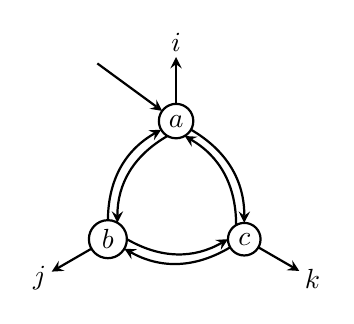
\begin{tikzpicture}[inner sep=2pt,outer sep=0pt,thick]
	\node[circle,draw] (a) at ( 90:1) {$a$} ;
	\node[circle,draw] (b) at (210:1) {$b$} ;
	\node[circle,draw] (c) at (330:1) {$c$} ;
	\node (i) at ( 90:2) {$i$} ;
	\node (j) at (210:2) {$j$} ;
	\node (k) at (330:2) {$k$} ;
	\begin{scope}[->,>=stealth]
	\draw (a.240) to[bend right] (b.60) ;
	\draw (b.0)   to[bend right] (c.180) ;
	\draw (c.120) to[bend right] (a.300) ;
	\draw (a.330) to[bend left]  (c.90) ;
	\draw (b.90)  to[bend left]  (a.210) ;
	\draw (c.210) to[bend left]  (b.330) ;
	\draw (a)--(i);
	\draw (b)--(j);
	\draw (c)--(k);
	\draw (120:2)--(a);
	\end{scope}
\end{tikzpicture}}}
\qquad
\begin{array}{l@{}l@{}l}
	S &~=~& \{a,b,c,i,j,k\}
\\[3pt]	s &~=~& a
\\[3pt]	F &~=~& \{i,j,k\}
\\[3pt]	\delta &~=~&  a \mapsto \D{~b./13~,~c./13~,~i./13~}
\\[3pt]            && b \mapsto \D{~a./13~,~c./13~,~j./13~}
\\[3pt]            && c \mapsto \D{~a./13~,~b./13~,~k./13~}
\end{array}
\]
Its interpretation is as follows, writing $\term{M+N+P}$ for the term $\termcolor\lfloor\D{M./13,N./13,P./13}\rfloor$.
\[
\begin{aligned}
	\sem C &~=~ \term{({\sem{C(b)}}+{\sem{C(c)}}+i)^a}
\\	       &~=~ \term{((a+{\sem{C(b)(c)}}+j)^b + (a+{\sem{C(c)(b)}}+k)^c+i)^a}
\\         &~=~ \term{((a+(a+b+k)^c+j)^b + (a+(a+c+j)^b+k)^c+i)^a}
\end{aligned}
\]
This term is typed as follows. As in the introduction, for brevity we omit return stacks from the types.
\[
\begin{aligned}
	    \term{(a+b+k)^c}         &: \type{\e => /13a + /13b + /13k}
\\[5pt]	\term{ a+(a+b+k)^c+j}~~~ &: \type{\e => /49a + /19b + /19k + /13j}
\\[5pt] \term{(a+(a+b+k)^c+j)^b} &: \type{\e => /12a + /18k + /38j}
\\[5pt] \term{(a+(a+c+j)^b+k)^c} &: \type{\e => /12a + /18j + /38k}
\\[5pt] \term{ (a+(a+b+k)^c+j)^b + (a+(a+c+j)^b+k)^c+i}~~~ &: \type{\e => /13a + /16k + /16j + /13i}
\\[5pt] \term{((a+(a+b+k)^c+j)^b + (a+(a+c+j)^b+k)^c+i)^a} &: \type{\e => /14k + /14j + /12i}
\end{aligned}
\]
The interpretation may be illustrated as follows, where the solid edges represent the tree-shape of the probabilistic sums, while the dashed edges represent the loops.
\[
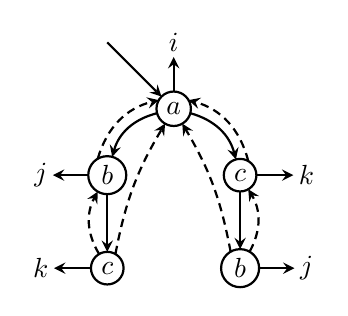
\begin{tikzpicture}[x=24pt,y=-24pt,inner sep=2pt,outer sep=0pt,thick]
	\node[circle,draw] (a) at (1,0) {$a$};
	\node[circle,draw] (b) at (0,1) {$b$};
	\node[circle,draw] (c) at (2,1) {$c$};
	\node[circle,draw] (d) at (0,2.4) {$c$};
	\node[circle,draw] (e) at (2,2.4) {$b$};
	\node (i) at (1,-1)   {$i$};
	\node (j) at (-1,1)   {$j$};
	\node (k) at ( 3,1)   {$k$};
	\node (l) at (-1,2.4) {$k$};
	\node (m) at ( 3,2.4) {$j$};
	\begin{scope}[->,>=stealth]
	\draw (0,-1)--(a);
	\draw (a) to[bend right] (b);
	\draw (a) to[bend left]  (c);
	\draw (a) -- (i);
	\draw (b) -- (d);
	\draw (c) -- (e);
	\draw (b) -- (j);
	\draw (c) -- (k);
	\draw (d) -- (l);
	\draw (e) -- (m);
	\begin{scope}[dash pattern=on 3pt off 2pt]
	\draw (b.120) to[bend left]  (a.150);
	\draw (c.60)  to[bend right] (a.30);
	\draw (d.120) to[bend left]  (b.240);
	\draw (e.60)  to[bend right] (c.300);
	\draw (d.60)  to[bend left=10]  (a.240);
	\draw (e.120) to[bend right=10] (a.300);
	\end{scope}
	\end{scope}
\end{tikzpicture}
\]
As the illustration suggests, the formalism may express any probabilistic tree with back-pointers. It may also express directed acyclic graphs, which yields a smaller interpretation of the Markov chain above, though still exponential, in the following term.
\[
	\term{ (b+c+i ; b -> a+c+j ; c -> (a+b+k ; b -> a+c+j)^c )^a }
\]
The types work out the same way.
\[
\begin{aligned}
	    \term{ b+c+i }~~~             &: \type{\e => /13b + /13c + /13i}
\\[5pt] \term{ b+c+i ; b -> a+c+j}~~~ &: \type{\e => /19a + /49c + /13i + /19j}
\\[5pt] \term{(a+b+k ; b -> a+c+j)^c} &: \type{\e => /12a + /18j + /38k}
\\[5pt] \term{ b+c+i ; b -> a+c+j ; c -> (a+b+k ; b -> a+c+j)^c}     &: \type{\e => /13a + /13i + /16j + /16k}
\\[5pt] \term{(b+c+i ; b -> a+c+j ; c -> (a+b+k ; b -> a+c+j)^c )^a} &: \type{\e => /12i + /14j + /14k}
\end{aligned}
\]


%----------------------------------------------------------------------------------------------------
\subsection{The first-order fragment is PAST}



%----------------------------------------------------------------------------------------------------
\subsection{AST vs PAST}

The following term $\term Z$ generates a geometric series of Church numerals.
\[
	\term{Z}~=~\term{ <f>.<x>.[x].~(<n>.~([n].*~+~[[n].f].i))^i ; <m>.m }~\sim~\D{\cno./12,~\cni./14,~\cnii./18,~\dots}
\]
Let $\term M=\term{<n>.([n].*~+~[[n].f].i)}$ so that the above term is $\term{ <f>.<x>.[x].M^i ; <m>.m }$. For a given $\term N$, the term$\term{[N].M^i}$ evaluates as follows.
\[
\begin{aligned}
\term{[N].M^i}  
 ~ \rws ~ & \term{[N].M;i->M^i}
\\    = ~ & \term{[N].<n>.([n].*~+~[[n].f].i);i->M^i}
\\  \rw ~ & \term{([N].*~+~[[N].f].i);i->M^i}
\\ \sim ~ & \term{[N].* ~+~ [[N].f].M^i}
\end{aligned}
\]
The overall term $\term{ <f>.M^i ; <x>.x }$ then generates the geometric series as follows.
\[
\begin{array}{@{}r@{}l@{}}
	       & \term{ <f>.<x>.[x].M^i ; <m>.m }
\\  ~\rws~ & \term{ <f>.<x>.([x].* ; [[x].f].M^i) ; <m>.m }
\\ 	~\sim~ & \term{ <f>.<x>.[x].<m>.m ~+~ (<f>.<x>.[[x].f].M^i ; <m>;m) }
\\  ~\rw ~ & \term{ \cno ~+~ (<f>.<x>.[[x].f].M^i ; <m>;m) }
\\  ~\rws~ & \term{ \cno ~+~ (\cni ~+~ (<f>.<x>.[[[x].f].f].M^i ; <m>;m)) }
\end{array}
\]
Church numerals allow exponentiation by $\underline{m^n}=\cnn\,\cnm$. The term $\term{[\cnii].Z}$ then generates the following series.
\[
	\term{[\cnii].Z}~\sim~\D{\cni./12~,~\cnii./14~,~\cniv./18~,~..}
\]
Since Church numerals are in unary notation, the terms in the series grow exponentially. Stochastically generating a Church numeral with $\term{[\cnii].Z}$ is thus almost-surely terminating, but not \emph{positively} so.

There are two minor caveats. First, the above computations use reduction $\rw$ and equivalence $\sim$, but not evaluation on the machine. Second, since the calculus encodes constants as choices, it only admits finite datatypes. One may address both issues by introducing a natural numbers type $\type\N$ with primitive operations $\term{`+:\N\,\N=>\N}$ etc. Then the following term evaluates on the machine to return a single natural number according to the above series. (This has been confirmed experimentally.)
\[
	\term{[[0].*].[<n>.n ; [1].`+].[\cnii].Z}
\]
Note that Church numerals $\term{\cnn}$ follow a call--by--name semantics, while primitive operations on natural numbers have a call--by--value semantics. This is reflected in the base value $\term{[0].*}$ and successor function $\term{<n>.n ; [1].`+}$, which incorporate the encoding of call--by--value into call--by--name. 

It remains to show that the above terms can be typed. First, for any type $\type{s=>t}$, and indeed any type $\type{!s=>!t_I}$, the Church numerals and the term $\term Z$ can be typed as follows.
\[
\begin{aligned}
	    \term{ n }                &: \type{s=>t}
\\[5pt] \term{ f }                &: \type{(s=>t)\,s => t}
\\[5pt] \term{ [[n].f].i }        &: \type{\e => (s=>t).i}
\\[5pt] \term{ [n].*~+~[[n].f].i} &: \type{\e => (s=>t)./12* + (s=>t)./12i}
\\[5pt] \term{M}~=~\term{<n>.([n].*~+~[[n].f].i)} &: \type{(s=>t) => (s=>t)./12* + (s=>t)./12i}
\\[5pt] \term{M^i}                &: \type{(s=>t) => (s=>t)}
\\[5pt] \term{Z}~=~\term{ <f>.<x>.[x].~M^i ; <m>.m } &: \type{((s=>t)\,s => t)~(s=>t)~s~=>~t}
\end{aligned}
\]
It follows that $\term{[\cnii].Z}$ can be typed with the same type. The types of the natural number constructions are as follows.
\[
	\term{[0].* : \e=>\N} \qquad
\qquad
	\term{<n>.n ; [1]. `+ : (\e=>\N)=>\N}
\]
This gives the following overall type. 
\[
	\term{[[0].*].[<n>.n ; [1].`+].[\cnii].Z : \e=>\N}
\]
The Church numeral types $\type{((s=>t)\,s => t)~(s=>t)~s=>t}$ of $\term{\cnii}$ and $\term{Z}$ here are specialised as follows: that for $\term{\cnii}$ by replacing $\type{s=>t}$ with $\type{\e=>\N}$, and that for $\term Z$ by replacing $\type{s=>t}$ with $\type{(\e=>\N)=>\N}$.
\[
\begin{aligned}
	    \term{\cnii} &: \type{((\e=>\N)=>\N)\,(\e=>\N)=>\N}
\\[5pt]	\term{Z}     &: \type{(((\e=>\N)=>\N)\,(\e=>\N)=>\N)~((\e=>\N)=>\N)~(\e=>\N)~=>~\N}
\end{aligned}
\]
The existence of this typed term gives the following.

\begin{proposition}
The probabilistically typed FMC expresses terms that are not positively almost-sure terminating.
\end{proposition}


%----------------------------------------------------------------------------------------------------

\bibliography{FMC-AST}

\end{document}


%====================================================================================================



